\documentclass[letterpaper]{article}
\usepackage{amsmath, amssymb, amsthm}
\usepackage[indent=16pt]{parskip}
\usepackage{graphicx}
\usepackage{hyperref}
\usepackage{tikz}
\usepackage{pgfplots}

\title{Flaky Tests in Software Development}
\author{Michael Hering}
\date{\today}
\pgfplotsset{compat=1.18} 

\begin{document}
\maketitle

\begin{abstract}    
    Test suites involving flaky tests can significantly increase the feedback loop duration and reduce confidence in application behavior. This paper analyzes the relationship between the number of flaky tests and both the probability of a successful build and the expected build duration. The results show that the probability of a successful build decays exponentially with the number of flaky tests, while the expected build duration grows exponentially. Maintaining a healthy build environment is essential for efficient and confident software development.
\end{abstract}

\section{Introduction}

Testing is a critical part of software development. It ensures that our applications behave as expected and catches unexpected changes early—before the application goes to production. Our testing systems are designed to be automated, fast, and continuous, with the goal of minimizing feedback cycle duration and maximizing confidence in our applications. 

We write automated test suites that run all tests at once, and we leverage continuous integration so that on each commit, a build is triggered which runs our test suites. If any single test fails, the build is failed entirely. This cycle creates rapid feedback which catches code issues before production and allows us to iterate on our applications with confidence.

However, in many test suites—especially those that depend on time, concurrency, or asynchronous processing for example—we encounter tests that sometimes pass and sometimes fail even without any changes to the code under test. These tests, known as \emph{flaky tests}, introduce false negatives into the build and have a compounding effect.

Teams may attempt to improve reliability by designing more complex CI systems which work around the issue by re-running specific steps of the build, or even only those tests which have failed. However, this strategy merely masks the problem and leads to a team which continues to introduce new flaky tests—ultimately leading to longer feedback cycles and reduced confidence in the application. 

Furthermore, it is important to note that while most flaky tests are false negatives—erroneously failing even when the code behaves correctly—there are instances where their intermittent behavior actually represents false positives, inadvertently masking a real bug that needs to be addressed. If we do not fix these tests right away, we may be shipping applications which contaion bugs.

Proactively addressing flaky tests as soon as they appear minimizes the compounding negative impact on the development lifecycle and application stability, leading to shorter feedback cycles, higher confidence in our applications, and a team that embraces rapid iteration. 

\section{Analysis}

A \textit{flaky test} is a test that sometimes passes and sometimes fails without any changes to the code under test. Here we analyze the relationship between the number of flaky tests and both the probability of a successful build and the expected build duration.

\subsection{Success Probability of a Single Build}

\setlength{\parskip}{1em}

Let \( n \) be the total number of flaky tests. Assume each flaky test has an independent probability \( p \) of failing on a given run.

For a single flaky test, the probability of passing is \( 1 - p \).

For \( n \) flaky tests, assuming that each build is an independent trial, the probability \( P \) that all \( n \) tests pass is:
\[
P = (1 - p)^n.
\]
As \( n \) grows larger:
\[
\lim_{n \to \infty} (1 - p)^n = 0.
\]
The probability of a single build being successful decays exponentially with the number of flaky tests.

\subsection{Total Build Duration}

If a build fails, it must be re-run until it succeeds. 

Let \( t \) be the duration of a single build run (e.g., \( t = 10 \) minutes) and recall that \( P = (1 - p)^n \) is the probability that a single build is successful. 

The number of build attempts \( X \) required until the first successful build follows a geometric distribution with expected value \(E[X] = \frac{1}{P}\).

Given that each build takes a fixed time \( t \), the expected total duration \( T \) to achieve a successful build is:
\[
T = t \cdot E[X] = \frac{t}{(1 - p)^n}.
\]
As \( n \) grows larger:
\[
\lim_{n \to \infty} T = \infty.
\]
The total build duration grows exponentially with the number of flaky tests.

\subsection{Numerical Examples}

Consider the following examples with \( p = 0.1 \) (i.e., a 10\% failure rate per test) and \( t = 10 \) minutes:

\textbf{1 Flaky Test:}
\[
P = 0.9, \quad E[X] \approx 1.11, \quad T \approx 11.1 \text{ minutes}.
\]

\textbf{4 Flaky Tests:}
\[
P = 0.9^{4} \approx 0.656, \quad E[X] \approx 1.52, \quad T \approx 15.2 \text{ minutes}.
\]

\textbf{16 Flaky Tests:}
\[
P = 0.9^{16} \approx 0.185, \quad E[X] \approx 5.40, \quad T \approx 54.0 \text{ minutes}.
\]

\textbf{64 Flaky Tests:}
\[
P = 0.9^{64} \approx 0.001, \quad E[X] \approx 841.6, \quad T \approx 8,481.6 \text{ minutes}.
\]

\begin{figure}[ht!]
    \centering
    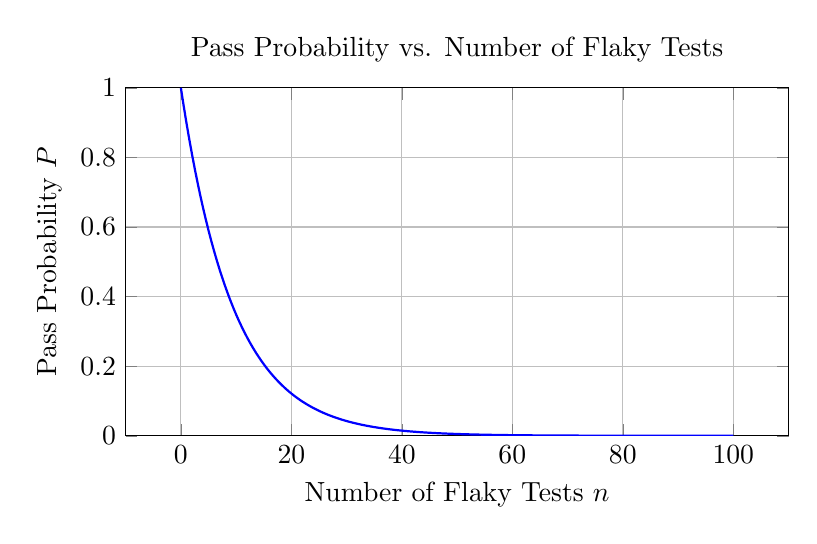
\begin{tikzpicture}
    \begin{axis}[
        title={Pass Probability vs. Number of Flaky Tests},
        ylabel={Pass Probability \( P \)},
        xlabel={Number of Flaky Tests \( n \)},
        ymin=0, ymax=1,
        domain=0:100,
        samples=200,
        width=10cm,
        height=6cm,
        grid=major
    ]
    \addplot[blue, thick] { (1-0.1)^x };
    \end{axis}
    \end{tikzpicture}
    \caption{As \( n \) grows, \((1-p)^n\) declines sharply from 1 to near 0. Even for a small \( p \) (e.g., 0.1), the probability of a completely passing build diminishes rapidly as \( n \) increases.}
\end{figure}

\pagebreak

\begin{figure}[ht!]
    \centering
    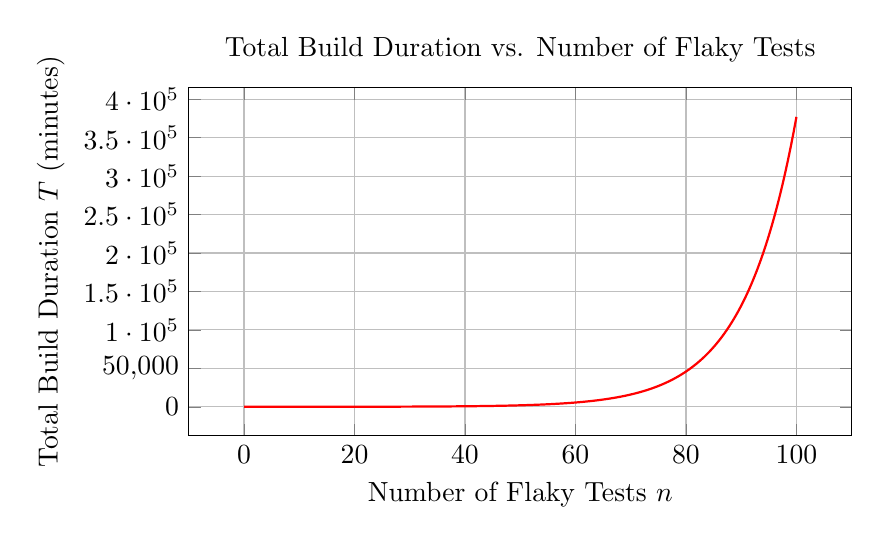
\begin{tikzpicture}
    \begin{axis}[
        title={Total Build Duration vs. Number of Flaky Tests},
        ylabel={Total Build Duration \( T \) (minutes)},
        xlabel={Number of Flaky Tests \( n \)},
        domain=0:100,
        samples=200,
        width=10cm,
        height=6cm,
        scaled ticks=false,
        grid=major,
        ytick={0, 50000, 100000, 150000, 200000, 250000, 300000, 350000, 400000},
    ]
    \addplot[red, thick] {10/((1-0.1)^x)};
    \end{axis}
    \end{tikzpicture}
    \caption{Total Build Duration increases exponentially with the number of flaky tests.}
\end{figure}

These examples illustrate how the expected number of builds—and thus the total build duration—increases significantly with the number of flaky tests.

\section*{Marginal Impact of Fixing Individual Tests}

There is an upside, however. When a flaky test is fixed, the improvement in pass probability depends on how many flaky tests remain. Fixing a flaky test when there are many will only yield a marginal improvement, but as the total number of flaky tests decreases, each fix results in a more significant increase in the overall build success probability. The following examples, where each test has \( p = 0.1 \) failure rate, illustrate this point:

\begin{itemize}
    \item Reducing the count from 64 to 63 flaky tests improves the pass rate from approximately 0.001 to 0.001 (a 0.01\% gain).
    \item Reducing the count from 16 to 15 flaky tests improves the pass rate from approximately 0.185 to 0.206 (a 2.1\% gain).
    \item Reducing the count from 4 to 3 flaky tests improves the pass rate from approximately 0.656 to 0.729 (a 7.3\% gain).
    \item Eliminating the last flaky test (from 1 to 0) improves the pass rate from 0.900 to 1.000 (a 10.0\% gain).
\end{itemize}

\begin{figure}[ht!]
    \centering
    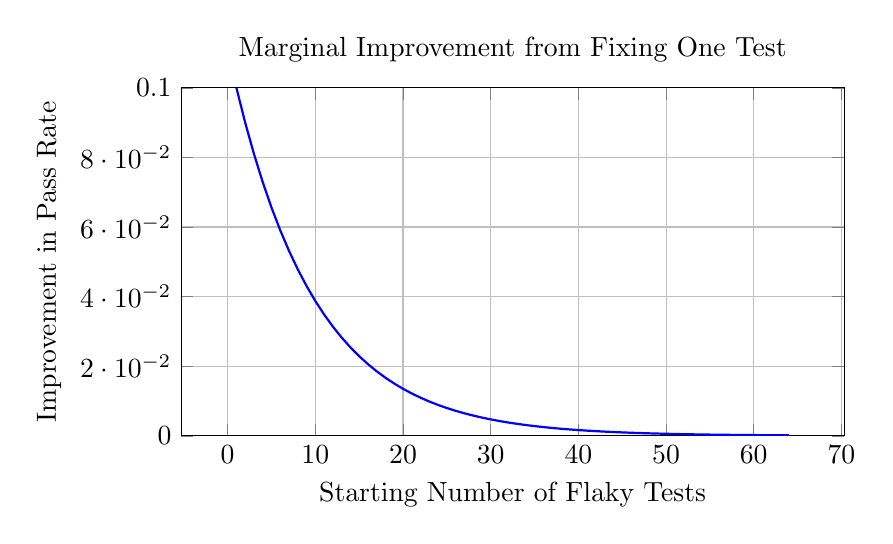
\begin{tikzpicture}
    \begin{axis}[
        title={Marginal Improvement from Fixing One Test},
        ylabel={Improvement in Pass Rate},
        xlabel={Starting Number of Flaky Tests},
        ymin=0, ymax=0.1,
        domain=1:64,
        samples=64,
        width=10cm,
        height=6cm,
        grid=major
    ]
    \addplot[blue, thick] {(0.9^(x-1))-(0.9^x)};
    \end{axis}
    \end{tikzpicture}
    \caption{The marginal improvement in pass rate when fixing one test, starting from \( n \) tests.}
\end{figure}

\section*{Conclusion}

Flaky tests create a compounding effect: even a small failure rate per test can lead to near-certain build failure and unacceptably long build times as more flaky tests are introduced. It is more efficient to address flaky tests as soon as they appear than to wait until many have accumulated. 

\end{document}
